% !TeX spellcheck = it_IT
\newpage
\section{Machine learning}
\subsection{Introduzione}
L'\textbf{apprendimento} è un principio universale per esseri viventi, per la società ma anche per le macchine. È permette di fornire l'\textbf{intelligenza} a sistemi. È un campo complesso ed in continua crescita per creare:
\begin{itemize}
	\item Computer che possano \textbf{imparare}
	\item Nuovi \textbf{strumenti} potenti ed adattivi con basi rigorose nell'informatica
\end{itemize}
Permettere alle macchine di imparare ci serve perché la quantità di dati sta aumentando esponenzialmente ed è molto difficile istruire una macchina solamente tramite istruzioni imperative.\\
Tra gli obiettivi ci sono:
\begin{itemize}
	\item Costruire \textbf{sistemi adattivi intelligenti} (e.g. robot, motori di ricerca)
	\item Creare \textbf{strumenti statistici} per analizzare i dati (data science)
	\item Affrontare \textbf{nuovi problemi} fin'ora troppo complessi (e.g. ambito medico)
\end{itemize}
\begin{example}[Email spam classification]
	\label{example:email_spam}
	Identificare tramite istruzioni rigorose quali mail sono o non sono spam è molto difficile, considerando anche che può variare da persona a persona. Il machine learning in questo caso permette di costruire una \textit{classificazione} basata su degli \textit{esempi} che si possa \textit{adattare} ai vari casi.
\end{example}
\begin{example}[Face recognition]
	Nel 2014 è stata sviluppata una rete neurale che permetteva, partendo dall'apprendimento di circa 4 milioni di immagini, di riconoscere le facce umane già viste, con una percentuale di successo del $97.25\%$ (quella umana è del $97.53$).
\end{example}
\begin{example}[Go]
	Il gioco del Go, in quanto molto complesso (anche più degli scacchi), si è adattato molto bene al machine learning, che con il tempo è riuscito a battere gli umani e a diventare sempre più esperto.
\end{example}
\begin{example}[Traduzione]
	Un'altra applicazione molto famosa sono i sistemi di traduzione automatica, come Google Translate dal 2016 o DeepL dal 2017.
\end{example}
\begin{example}[Medicina]
	Il machine learning in ambito medico può aiutare in diversi aspetti: dalla diagnosi alla terapia, alle medicine personalizzate, al monitoraggio della salute e persino alla progettazione delle medicine stesse.\\
	Uno degli esempi più famosi è quello della rete neurale che permette di riconoscere il cancro alla pelle con l'accuratezza di un dermatologo certificato.
\end{example}
\begin{example}[Musica]
	Anche nell'arte, in particolare della musica, ci sono diversi esempi di Machine Learning, come AIVA, una rete neurale che è partita dalla composizione di un brano per pianoforte ed è arrivata ad orchestre e colonne sonore per videogiochi.
\end{example}
\begin{note}[Premio Turing]
	Il premio Turing del 2018 è stato vinto da tre professori, il Dr. Hinton, il Dr. LeCun e il dottor Bengio, per il loro lavoro innovativo che ha reso le reti neurali profonde un componente fondamentale per l'informatica moderna.
\end{note}

\subsubsection{Quando?}
Il machine learning deve essere utilizzato quando può essere \textbf{utile} (\textbf{opportunity}):
\begin{itemize}
	\item Per problemi di cui c'è poca o nessuna teoria
	\item In presenza di dati incerti, distorti o non completi
	\item In ambienti dinamici che non possono essere previsti in anticipo
\end{itemize}
e con criterio in base a ciò di cui ha bisogno (\textbf{awareness}):
\begin{itemize}
	\item Una fonte di apprendimento
	\item Si deve accettare che i risultati avranno una certa tolleranza
\end{itemize}

\begin{note}
	Il machine learning non è una metodologia approssimata ma bensì un metodo rigoroso per trovare una funzione approssimata che gestisca il problema complesso. Viene quindi definito \textbf{soft computing}, ovvero aperto a nuove possibilità (e.g. la biologia).
\end{note}

\subsection{Sistema predittivo}
Un sistema si compone dai \textbf{dati}, ovvero le osservazioni del mondo reale, da un \textbf{modello}, che può migliorare tramite apprendimento ed è quindi composto anche da \textit{task}, \textit{algoritmo di apprendimento} e metodo di \textit{validazione}, e da una \textbf{previsione}. 
\begin{center}
	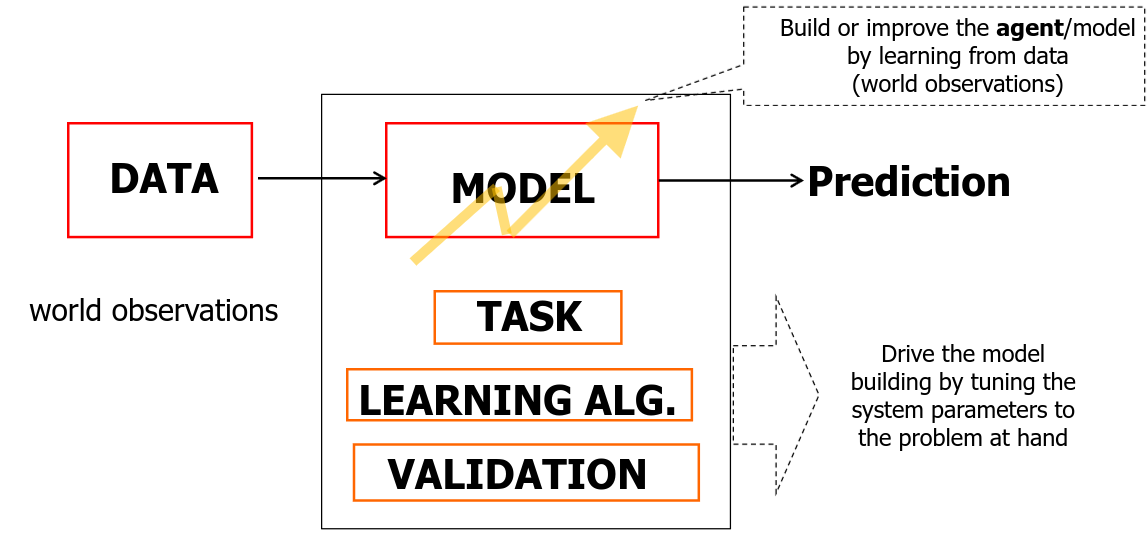
\includegraphics[scale=0.4]{predictive_system.png}
\end{center}

Il machine learning consiste nel ricostruire una \textbf{funzione} a partire dai dati.
\begin{example}[Riconoscimento della scrittura]
	Partiamo dai dati in \textbf{ingresso}: una raccolta di immagini di scrittura a mano di cifre sotto forma di array e matrici. Vogliamo costruire un modello che, ricevuta in input un'immagine di scrittura a mano, ne predica le cifre.
	
	\begin{center}
		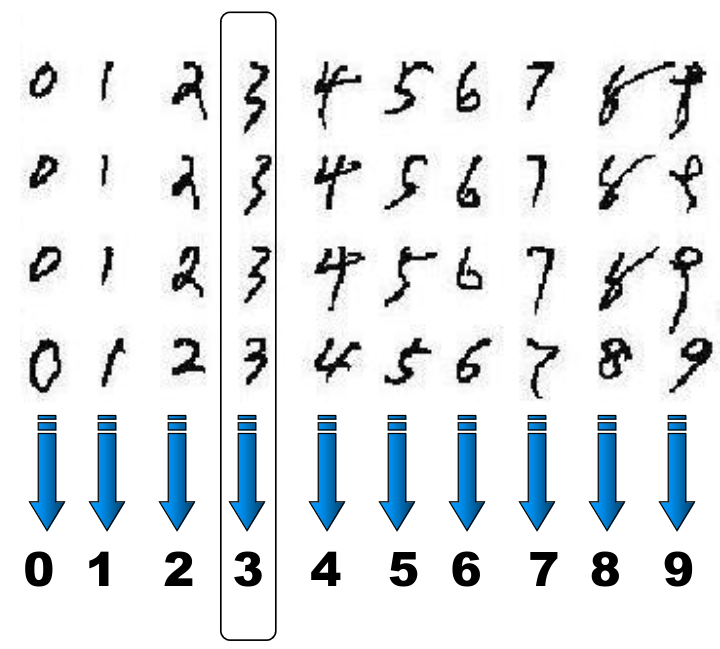
\includegraphics[scale=0.2]{hand_writing_recognition.png}
	\end{center}
	Il problema ha quindi una soluzione difficile da formalizzare (presenza di rumore e ambiguità nei dati) ma è facile ottenere dei dati da cui far apprendere il modello.\\
\end{example}

L'apprendimento può essere di due tipi:
\begin{itemize}
	\item \textbf{Supervisionato}: a partire da una serie di dati \textbf{supervisionati} (sappiamo che etichetta hanno), si crea una funzione che si possa applicare ad altri casi
	\item \textbf{Non supervisionato}: a partire da una serie di dati non etichettati cerchiamo \textbf{raggruppamenti naturali} come:
	\begin{itemize}
		\item Clustering
		\item Modellazione della densità dei dati
		\item Preprocessing, visualizzazione, riduzione dimensionale
	\end{itemize}
\end{itemize}

\subsubsection{Apprendimento supervisionato}
\begin{definition}[Task]
	Dato un insieme di \textbf{esempi} etichettati del tipo
	\begin{equation*}
		<input,output>=(\textbf{x},d)
	\end{equation*}
	per una \textbf{funzione} sconosciuta $f$, di cui conosciamo il valore solo per i punti in ingresso (\textbf{target value} $d$).\\
	Dobbiamo trovare una buona \textit{approssimazione} a $f$, ovvero un \textbf{ipotesi} $h$ che può essere usata per fare previsioni su dati mai visti $x'$.\\
	Il \textbf{target} può essere:
	\begin{itemize}
		\item \textbf{Categorico} per i problemi di \textbf{classificazione}: $f(\textbf{x})$ restituisce la presunta corretta classe tra $\{1,2,\ldots, k\}$
		\item \textbf{Numerico} per i problemi di \textbf{regressione}, dove $f(\textbf{x})$ restituisce valori continui
	\end{itemize}
\end{definition}

\begin{example}
	Alcuni esempi di funzioni:
	\begin{itemize}
		\item Riconoscimento di scrittura
		\begin{itemize}
			\item $\textbf{x}$: dati dalle immagini dei caratteri
			\item $f(\textbf{x})$: lettere dell'alfabeto
		\end{itemize}
		\item Diagnosi di malattie da cartella clinica
		\begin{itemize}
			\item $\textbf{x}$: dati sul paziente (sintomi, analisi di laboratorio)
			\item $f(\textbf{x})$: malattia o terapia consigliata
			\item Training set: cartella clinica del paziente
		\end{itemize}
		\item Riconoscimento facciale
		\begin{itemize}
			\item $\textbf{x}$: immagine della faccia della persona
			\item $f(\textbf{x})$: nome della persona
		\end{itemize}
		\item Riconoscimento dello spam
		\begin{itemize}
			\item $\textbf{x}$: email
			\item $f(\textbf{x})$: spam o non spam
		\end{itemize}
	\end{itemize}
\end{example}

\begin{definition}[Modello]
	Un modello ha come obiettivo quello di descrivere le relazioni tra i dati sulla base di un task. Definisce la classe della funzione che la macchina può implementare, ovvero lo \textbf{spazio delle ipotesi} (e.g. $h(\textbf{x}, \textbf{w})$ dove $w$ sono parametri astratti).
\end{definition}
\begin{definition}[Esempi di training]
	Un esempio della forma
	\begin{equation*}
		(\textbf{x}, f(\textbf{x})+noise)
	\end{equation*}
	dove $\textbf{x}$ è di solito un vettore di caratteristiche e $d=f(\textbf{x})+noise$ è il \textbf{target value}.
\end{definition}
\begin{definition}[Funzione obiettivo]
	La vera funzione $f$.
\end{definition}
\begin{definition}[Ipotesi]
	Una proposta di funzione $h$ che si crede essere simile a $f$. Un'espressione in un determinato \textbf{linguaggio} (e.g. logico, numerico o probabilistico) che descrive la relazione tra i dati.
\end{definition}
\begin{definition}[Spazio delle ipotesi]
	L'insieme di tutte le ipotesi che possono in teoria essere date in output dall'algoritmo.
\end{definition}

\noindent Alcuni modelli sono:
\begin{itemize}
	\item Modelli \textbf{lineari}, dove ogni rappresentazione di $h$ definisce uno spazio continuo di ipotesi. Ogni assegnamento di \textbf{$w$} è un'ipotesi differente. Ad esempio
	\begin{equation*}
		h_w(x)=w_1x+w_0 \quad h_w(x) = 0.232x + 246
	\end{equation*}
	\item \textbf{Regole simboliche}: lo spazio delle ipotesi è composto da rappresentazioni discrete. Si possono applicare diverse regole, ad esempio:
	\begin{lstlisting}[language=Python]
		if (x_1=0) and (x_2=1) then h(x)=1
		else h(x)=0
	\end{lstlisting}
	\item Modelli \textbf{probabilistici}: si fa una stima di $p(\textbf{x},y)$
	\item Modelli basati su \textbf{istanze}: predicono il valore medio $y$ dei vicini più prossimi (memory based)
\end{itemize}

\begin{definition}[Algoritmo di apprendimento]
	È un algoritmo che si basa sui dati, sulle task e sul modello ed impara con una ricerca euristica attraverso le ipotesi nello spazio $H$ delle migliori ipotesi (di solito cercando $h$ con l'errore minimo che si approssimi meglio alla funzione obiettivo).
	\begin{center}
		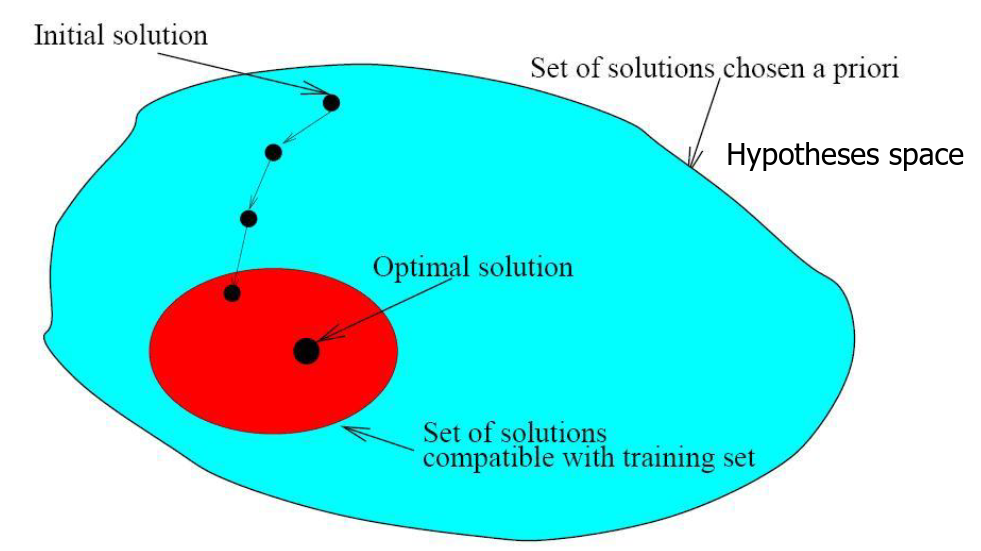
\includegraphics[scale=0.2]{learning_alg_search.png}
	\end{center}
\end{definition}

\begin{note}
	L'insieme $H$ potrebbe non coincidere con tutte le possibili funzioni e la ricerca quindi non può essere esaustiva: deve fare determinate assunzioni.
\end{note}

\begin{definition}[Funzione buona]
	Definiamo una funzione trovata come buona se è \textbf{generale}, ovvero in base a quanto è accurata nel predire i valori per nuovi dati. Ci sono quindi due fasi:
	\begin{itemize}
		\item \textbf{Learning}: il modello viene costruito da dati noti
		\item \textbf{Test}: il modello viene applicato a nuovi esempi e vengono valutate le capacità predittive in maniera \textbf{generale}
	\end{itemize}
\end{definition}
\begin{note}[Performance]
	Nel Machine Learning la performance indica l'accuratezza del modello nel predire un risultato, stimata dall'errore computo nella fase di test.
\end{note}